\section{Strategy}

\subsection{Cooperative Rabin-Karp}
\begin{frame}
	\frametitle{Definition}
	\begin{itemize}
		\item We define $\mathcal{S}$ and $\mathcal{T}$ vectors 
		as follow:
	\end{itemize}
	\begin{figure}
		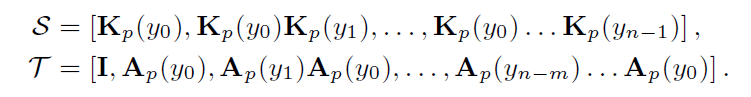
\includegraphics[scale=0.50]{figure/fig-ST.png}
	\end{figure}
	\begin{itemize}
		\item With $p$ processors, a scan can be computed in 
			$O(n/p + \log p)$ time steps.
	\end{itemize}
\end{frame}


\begin{frame}
	\frametitle{Final Result}
	\begin{figure}
		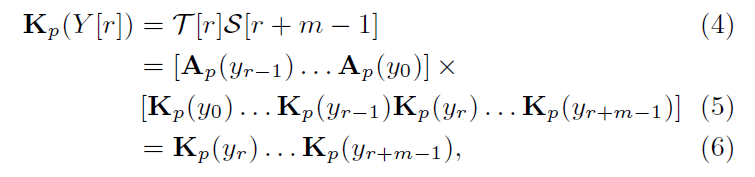
\includegraphics[scale=0.50]{figure/fig-Kp.png}
	\end{figure}
	\begin{itemize}
		\item Scan operation can be computed cooperatively by a set of 
		independent threads or processors.
	\end{itemize}
\end{frame}

\subsection{Divide-and-Conquer Rabin-Karp}
\begin{frame}
	\frametitle{Divide and Conquer}
	\begin{itemize}
		\setlength\itemsep{1em}
		\item These parallel scans require intermediate communication
		 between different processors and cores.
		\item Assign different parts of the text of different 
		processors and process each part seperately. The final result
		is simply a union of matching results for each subproblem.
	\end{itemize}
\end{frame}

\begin{frame}
	Let $L$ denote the number of subtexts. Then, if we
	show each subtext as $Y^l$, for $0 \le l < L$, the division
	process can be shown as:
	\begin{figure}
		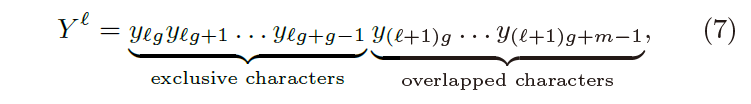
\includegraphics[scale=0.50]{figure/fig-DC.png}
	\end{figure}
	where each subtext has $g = (n-m+1)/L$ \textit{exclusive} 
	characters, plus $m-1$ \textit{overlapped} characters.
	\begin{itemize}
		\item If $L = 1$, DRK will be identical to CRK.
	\end{itemize}
\end{frame}

\subsection{Hybrid Rabin-Karp}
\begin{frame}
	\begin{itemize}
		\setlength\itemsep{1em}
		\item We define \textit{Hybrid RK} (HRK) as a method in which 
		the main text is divied into subtexts (Eq. (7)) and then each 
		subtext is assigned to a group of processors.
		\item If $L = 1$, HRK will be identical to CRK.
	\end{itemize}
\end{frame}

\begin{frame}
	\begin{figure}
		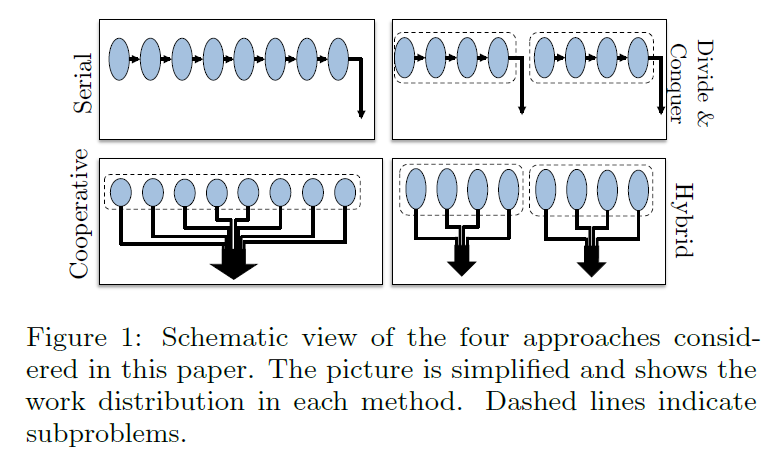
\includegraphics[scale=0.50]{figure/fig-all.png}
	\end{figure}
\end{frame}

\subsection{Theoretical Analysis}
\begin{frame}
	\frametitle{Theoretical Analysis}
	\begin{itemize}
		\setlength\itemsep{1em}
		\item The finite number of $p$ processors.
		\item Assume that all processors have access to a globally 
		shared memory.
	\end{itemize}
	\begin{figure}
		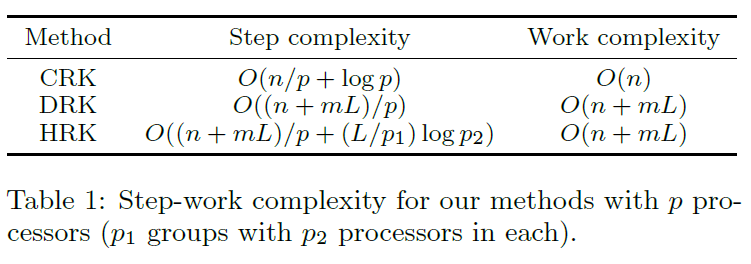
\includegraphics[scale=0.40]{figure/fig-complexity.png}
	\end{figure}
\end{frame}

\begin{frame}
	\frametitle{Theoretical Conclusions}
	\begin{itemize}
		\item We expect to see an approximate linear increase in the running time of all our parallel alternatives.
		\item CRK is superior to the other algorithms, and for all
		larger patterns.
	\end{itemize}
	\begin{figure}
		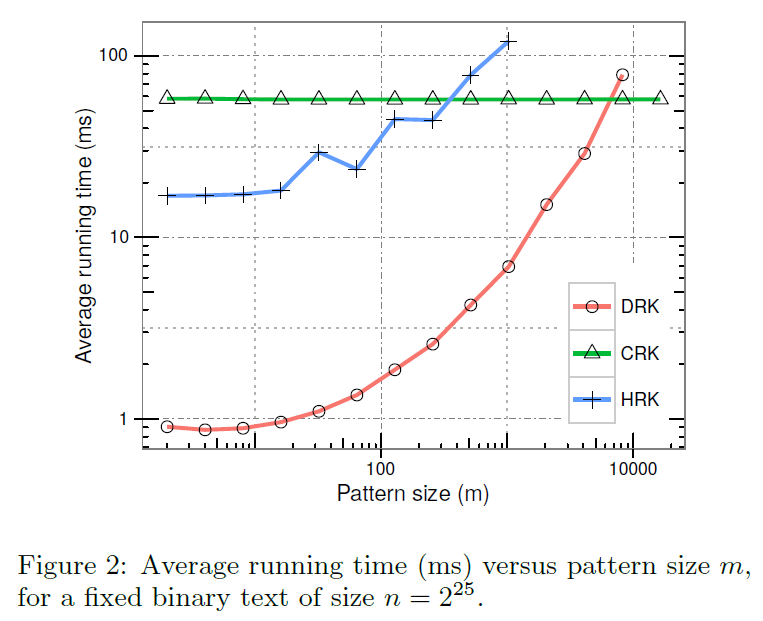
\includegraphics[scale=0.25]{figure/fig-result.png}
	\end{figure}
\end{frame}